\startchapter{Making Socio Technical Congruence Actionable}
\label{chap:actionable}
This Chapter concludes the work of this thesis by exploring the final research question \textbf{RQ 2.4:} \emph{Can recommendations be given in a timely manner?}
To explore this final question we first present how such a recommender system might look like to motivate its potential usefulness and continue with describing our study in a student course setting to answer our final research question.

\section{Recommender System: Chat To Succeed}
\label{chap:making:sec:cts}
Most software projects have infrastructure in place that automatically builds the software system on a regular basis. 
If there are errors in this build, if automated regression tests fail, or if a developer finds a major flaw in a build this build is considered as a failed build.  
Research shows that communication structures can be used to predict the outcome of a build~\cite{wolf:icse:2009}.  
Certain patterns of communication among team members who contribute to the code can determine if a build fails or succeeds. 
We expand this idea by providing specific recommendations of who should chat together to ensure a successful build.

We showed in Chapter~\ref{chap:stc-net} evidence that a build might fail due to a possibility that members of the software team coordinated poorly between the time the current build broke, and the last known successful build. 
One possible reason for this lack of coordination is that the team members who worked on interrelated components failed to inform each other about their changes. 
This brings us to the discussion of socio-technical congruence.

\subsection{Socio-technical Gaps}
Socio-technical congruence defines the match of technical and social dependencies among people, for example tasks (technical) and task related communication (social)~\cite{cataldo:cscw:2006}. 
It compares a technical network to a communication network and identifies gaps where a coordination need exists, but no communication fills the gap. 
We showed that gaps have a negative influence on the project~\cite{} as well as that there are specific gaps that correlate to build failure~\cite{}. 

\begin{figure}[t]
\centering
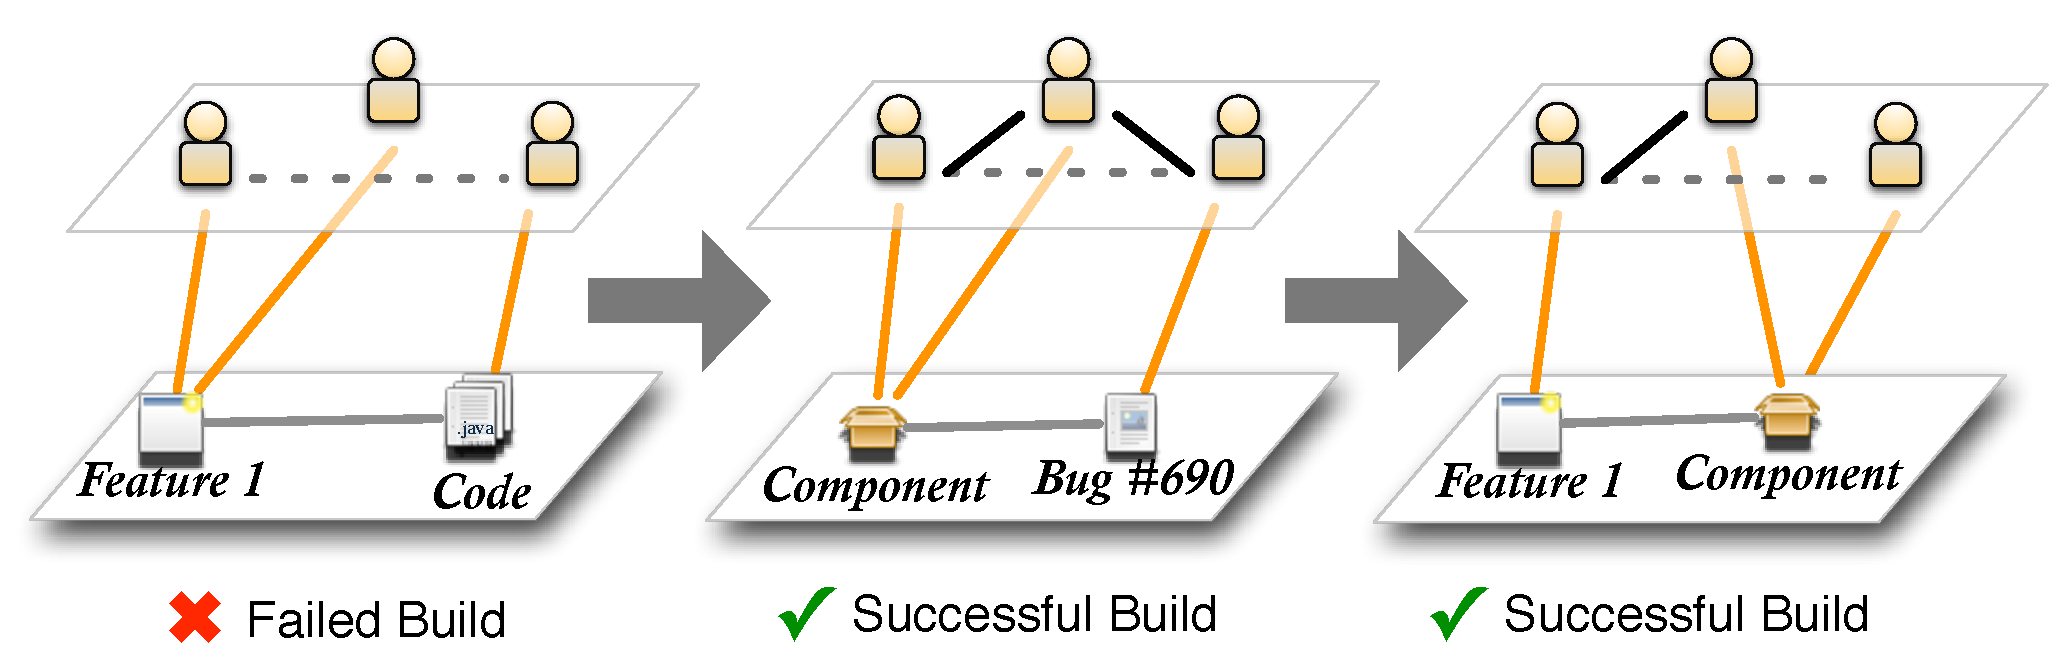
\includegraphics[width=0.9\columnwidth]{figures/bad-to-good}
\caption{Identifying failure inducing coordination gaps.}
\label{fig:multipleplanes}
\end{figure}

\subsection{Our Recommender System}
A recommender system based on socio-technical congruence gaps to prevent a failed build will identify which gaps are most likely to induce build failures. 
Figure~\ref{fig:multipleplanes} shows the social and technical networks for three builds. 
Developers are connected by working on the same artifact and by dependent artifacts. 
We see that the failed build exposes two socio-technical gaps. 
A first glance, this might lead to the conclusion that these gaps are related to build failures. 
Further examination of the two following successful builds suggests that only one gap is bad since the other gap exists in one of the successful builds as well. 
To generate our recommendations we connect people in two ways: (1) on the technical level and (2) at the social level. 

\begin{description}
\item[Technical Level.] 
We mine repositories such as tracking systems and code for technical connections. 
For example, two developers have a technical connection if they work on dependent components or related bug fixes.
\item[Social Level.]
Social level connections can be found by mining email, chat, or comments~\cite{cataldo:cscw:2006}. 
In particular we need to focus on the tasks that are represented by the mined technical connections. 
\end{description}

We could draw data from repository system by IBM called Jazz, which stores issue tracking, source code, and change sets in a single database. 
Jazz records associations between work items and change sets, as well as the results of integration builds. 
A build, therefore, includes the code contributions between the current integration build and the previous integration build. 
Thus, we can identify who has contributed to each integration build and who has coordinated about change sets that were included in a particular build.

We also draw data from open-source projects. 
In an open-source project that does not use Jazz, we can identify change sets from their source code repositories, and corresponding tracker items or development mailing list items based on commit logs. 
Prior to the data mining, the project's development system must be studied and understood in order to provide good recommendations.

\section{A Course on Globally Distributed Software Development}
To answer our final research question for this thesis \textbf{RQ 2.4:} \emph{Can recommendations be given in a timely manner?} we conduct a case study together with students taking a class in globally distributed software development.
The reasoning for choosing this student course as the basis for exploring our final research question has several reasons:
\begin{itemize}
\item Providing a project infrastructure that supports data collection.
\item The distribution of the course across countries ensures a minimum at electronically recordable and mineable communication data being generated.
\item A course setting allows for more control to ensure data quality.
\item A course setting enables better access to study participants.
\end{itemize}

One key to explore our research question is to collect data to analyze.
In a course project we are able to choose and instrument the infrastructure used by the students to actively develop software and thus possible gain more insight or at least miss less data than in most industrial settings that rarely focus on collecting data for analysis.
This especially allows us to establish traceability links between artifacts that are often missing and need to be inferred using semi-accurate heuristics.

Furthermore, the distributed nature of the project makes synchronous non-text based communication more difficult and thus increasing the use of text based asynchronous, and therefore recorded, communication.
This additional need to rely and flexible and stable communication media, mainly email and text based chats, enables us to collect more data that is easier to mine than it would have been realistic in a collocated setting.
The distributed nature of the teams, also induced an openness to work in a more distributed fashion even among collocated team members due to a sensibilisation of trying to enable their remote team members to follow their discussions.

Due to the nature of the study being conducted in a course setting, we had more control about how participants are using technology and could give guidance on how to improve their collaboration through means that are easy to record.
Because participants need to attend lectures we can educate them in a way that emphasizes the importance of recording traceability links in an searchable format.

Since the participants are students taking a class on software development, we can more easily arrange for time to give feedback on the study in the form of the quality of data that we are collecting and the collections method influence on the development process.
This feedback loop enables us to change the data collection to accommodate the needs of the students more easily and therefore ensure data quality by mitigating the risk of participants neglecting the data collection process. 

In the next section we provide a more in-depth description of the study setting and the data that we expect to collect.

\section{Setting}
\subsection{Course Details}
The globally distributed software development course taught at both the University of Victoria, Canada, and Altoo University, Finland, aims at teaching students how to develop software in a distributed setting.
In this particular course student teams where forced to deal with the issues that come with a distributed team in an extreme way since both West Coast Canada and Finland are separated by a time difference of 11 hours minimizing the time all team members are awake.
This both necessitates and motivates the students to apply lessons learned in the class room as for most of the students this situation is unfamiliar.

The course on globally distributed software development took place starting in October 2011 and ended in April 2012.
With the Finnish students starting in October 2011 and the Canadian students joining the development effort in Januaray 2012.
This further allowed the students to engage in remote collaboration as the Finish students represent the experts on the system the teams are working on and will need to guide their Canadian teammates in getting used to the projects layout and functions.

Besides developing a software product the Canadian students also have regular classes.
During a regular class the students participate in a seminar style setting that requires each student to read a set of papers, that can be discussed on the course blog, and discuss implications of the findings detailed in the papers and how these findings may apply to their current development experience.
Every two weeks the seminar style class is interrupted for a project wide meeting to bring together all the teams, including the Finish team members, to show case their progress and to plan the next steps and for the following two weeks.

The students filled out a survey every other week giving feedback on the class, the development process, and the use of different tools for communication and development.
Besides this bi-weeklu survey the students also had the chance to talk to the course instructors as well as the teaching assistant to issue concerns and make suggestion on how to improve the course for the students as well as issues they see with the quality of the collected or non-collected data.

\subsection{Team Composition}
As described earlier each development team consists of both students from Canada and Finland.
There are three teams with each team consisting of four students from Canada and two students from Finland.

In addition to the three teams we also have a product owner of software product that came up with the idea of the product, that we will describe in greater detail in Subsection~\ref{chap:make:subset:devproject}.
The product owner is located in Finland and is responsible for prioritizing the different features that he wants to be implemented.
Moreover, he negotiates with the teams what items they should aim for within a given two week span. 

To coordinate the work across teams, one Finish student has become the scrum master or de-facto project manager.
He is both the most experienced developer as well as has the most knowledge about the projects he is using the product within his own company.
Facilitating coordination across teams entails setting up meeting between team members as well as structuring the biweekly project meeting.
He also takes care of scoping out development tools to use and ensures that everyone is up to speed with issues arising from other teams that may implicate their work.

\subsection{Development Project}
\label{chap:make:subset:devproject}
The students in this course are extending the agile-planning tool agilefant\footnote{www,agilefant.org}.
Agilefant combines task creation, management, and planning into one tool that allows both to schedule different tasks for different sprints, with a sprint being a time period that is meant to implement a fixed set of tasks.
Furthermore, tasks can be organized hierarchically and be of different types, such as user stories or bug reports.
 
As mentioned previously, this product was conceived by the product owner and has since been developed by students participating in cap-stone projects at Altoo University, Finland.
The tool itself is open source and available to any one to download, install and extend as they see fit.

Besides being a student driven project it found a number of users in industry.
Due to the development being mainly undertaken in the cap-stone projects that are offered yearly to the students, the project progresses in spurts instead of gradually.
Nevertheless, the stability of its core feature and light weight approach it is popular among small and mid-sized companies to plan their development.

\subsection{Development Process}
The project follows a scrum process~\cite{} and thus development progresses in small sprints working of a common backlog.
A sprint, in the case of our project, is defined to be two weeks long starting with a planning session and ending in a retrospective.
The planning sessions and retrospectives take place between two sprints at the same day starting with the retrospective followed by the planning for the next sprint.

\subsection{IT-Infrastructure}
The source code is managed using GIT\footnote{http://git-scm.com/} and is available on github.com\footnote{https://github.com}.
Although Agilefant or github.com issues can be used for task management both are missing important features, github.com is missing the planning capabilities of a full agile planning tool and Agilefant is missing the ability to discuss work items.
Therefore, we use IBM Rational Team Concert for the planning of sprints and tracking of work items.
An additional advantage of IBM Rational Team Concert it is integrating with Eclipse the main development environment, which also integrates with git. 

Besides using discussions on work items, the students also use email and irc for communication.
To ensure that everyone has the same knowledge students are encouraged to summarize their email and irc discussion in work item discussion.
For group meetings especially the planning and retrospective session we provided the student with separate rooms and internet access to use google hangout for video chatting and screen sharing when discussing their group individual sprint plans.
For the project meeting after each sprint to demo their accomplishment to the development team at large, we provided conferences room with multiple microphones and screens to simultaneously show a number of remote participants as well as screen sharing sessions. 

To further support the development process the students set up a Jenkins an open source web-based build system.
This build system allows for continuous testing and thus help the students to get a better understanding of their progress with respect to implementing their tasks for a given sprint.

\section{Background and Related Work}
Socio-technical congruence builds the basis for our recommendation generating approach detailed in the previous Section~\ref{chap:making:sec:cts}.
Measuring the overlap between social relations, as represented by the communication among developers, and technical relations, as represented by artifact dependencies, socio-technical congruence shows a relation between build success and maximum coverage of technical relations by social relations~\cite{}.

Traditionally socio-technical congruence research focused showing that better adherence to Conway's law~\cite{} results in higher productivity~\cite{}.
We and others showed that additionally to the relation with productivity socio-technical congruence also has an affect on software quality.  

Although socio-technical congruence has the potential to generate recommendations that can be used to prevent failures (as detailed earlier in Section~\ref{chap:making:sec:cts} and Chapter~\ref{chap:stc-net}), it currently lacks in its actionability to utilize the insights produces so far.
In the calculation of socio-technical congruence, or to be more precise, in building the technical networks, the knowledge about technical relationship as created by change-sets is needed.
Since a change-set is only known once it has been submitted and thus the work has already been done, there is a need to approximate a change-set before all the work has been done.

Blincoe et al~\cite{} tackled this issue by using traces generated by Mylyn~\cite{}, a tool that help developer to focus on recently selected and edited source code, and to enable other to retrace their steps to accomplish a task.
They found that using these Mylyn traces to highly accurate in approximating the congruence metrics calculated using change-sets.
Furthermore, proximity can accurately predict coordination needs before before the completion of a change-set and, thus, is bale to be used to generate actionable knowledge.

\section{Methodology}
\subsection{Proximity to Infer Real Time Technical Networks}
\label{chap:making:subset:proximity}
In order to be able to explore the possibility of recommending improvements with respect to the socio-technical networks, we need to be able to intervene before the majority of work has been done.
The main issue with creating real time socio-technical networks lies with constructing technical networks as they are only known once a developer submits her changes to a repository.
On the other hand social-networks can be more readily constructed in real time because in order to communicate, at least electronically, will yield a trace for each bit of communication traveling from one person to the other and thus allow to extend a social network with each new instance of communication.

To gain a similarly effective way to construct technical network we build upon the work of Blincoe et al~\cite{}, who proposed a measure called proximity using Mylyn~\cite{} traces to infer real time developer dependencies.
Mylyn is an Eclipse plug-in that records edits and selects within source code files.
These event show which artifacts have been modified and selected thus allow the partial construction of a technical network based on ownership information of the modified, selected, and implicated source code artifacts.

In order to record this information in real time in a central repository we developed a plug-in that is capturing events recorded by Mylyn, connecting them to the current task a developer is working on, and submitting this information to a central server. 
To encourage students further to install this plug-in, we also provided a visualization of the current proximity of a developer to any other developer given her current task in a visualization plug-in called ProxiScentia~\cite{}.

\subsection{Data Collection}
For our study we collect six types of data:
\begin{itemize}
\item Communication data such as e-mails, irc chat logs and work item discussions.
\item The source code repositories on github.com, including each developers fork of the main repository.
\item Log of the build engine indicating failed and successful builds.
\item Documentation and diaries created by students during the course.
\item Surveys and questionnaires completed by students throughout the course. 
\item Mylyn events gathered using our custom build Eclipse plug-in.
\end{itemize}

Although we are not necessarily interested in constructing social networks for this part of the study but rather we are concerned whether it is possible to prevent build failures given a certain set of collectible data, we need access to as much communication data as possible not only as a means to see what kind of problems arose and whether they were of any importance to the developers.
For example, are build failures a problem for the developers and as such are all build failure equal.
Knowing which build failure are actually problematic to the developers lets us focus on those instances that do matter.

To further the investigation into the issues reported by the developers we make use of the version control systems used.
In our case these are several git repositories hosted on github.com.
Each developer owns her own forked repository from which she pushes changes to her respective team repository.
Once a feature implementation or bug fix has been reviewed by the product owner it is pushed to the project repository to ensure that each development team and team members is working on the latest stable code.

Since implementing quality features was a main concern during the class, the students set up a build-engine to continuously test their implementations.
Jenkins\footnote{}, the build engine used by the teams, keeps a log of all the builds as well as their outcomes.

Besides collecting data that is generated by the development activities of the students during the course we also asked them to keep a development diary as well as fill out frequent surveys that gauge their impression of the progress within the project as well as the adequacy of the tools used.

Finally, as mentioned in the previous Subsection~\ref{chap:making:subset:proximity} we also collect the code interactions with respect to which methods in the source code have been edited or selected in a central repository.

\subsection{Analysis}
Our analysis of for determine the feasibility of creating predictions based on socio-technical networks.
We go over data collected during the course in six steps, starting from identifying issues of interested to showing how recommendations based on our framework could have avoided these build failures:

\begin{enumerate}
\item Identify build issues mentioned by the developers.
\item Identify the actual failed build in the Jenkins build logs.
\item Identify the code changes that contributed to the build failure.
\item Check if the recorded code interactions could have predicted the build failure.
\item Check if the relation between the code changes could have predicted the build failure.
\item Check if using the social-network help findings the right people to include in order to resolve the issue.
\end{enumerate}

\paragraph{Identifying build issues.}
To find build issues that are truly build issues to the developer and not only such that report as a build failure due to test cases that failed and were meant to fail, we code the communication with respect to problems experienced in the project.
From those coded problems we select all problems related to building the software.

\paragraph{Identifying the actual failed build.}
After we identified from all the recorded communication what failed builds are truly failures, we identify those builds as they are shown in the Jenkins logs.
These builds show what went wrong as well as what changes are new to those builds that potentially broke it.

\paragraph{Identify code changes.}
Knowing the code changes that newly went into a build and consequently made it fail, are important to now as we need to use those change-sets to determine which interaction history to investigate.
From the change set we can determine the task worked on, as we require every student to annotate each submitted change-set with work item id the change-set was meant to implement.

\paragraph{Check code interactions}
Having the change-sets and thus the work items the developers worked on, enables us to retrieve the specific code interactions associated with that tasked produced by the developer that submitted the possibly offending change-set.

\paragraph{Check change relations.}
Knowing both, the change-set as well as the interaction traces that where involved in the failed build, we can contrast and overlay those change-sets as well as code interactions to see if the path of different developers overlap in way that let's us predict the issues we observed.

\paragraph{Check social network}
In case we see observe that the code traces that we collected could have predicted the issue, we look for cues in the communication media for the resolution of the issues and see if the knowledge about the code traces and the communication happening at the time of implementing the change-set.
Finding a relation between the code interactions and the ongoing communication during the implementation contrasted with the communication needed to resolve the issue create by the change-set is the key to building a useful recommendation.

Instead of analyzing each build failure that is important to the developers, we focus on finding one build that let's us trace the error back to the code interactions as well as shows a connection between the code interactions and the communication needed to resolve the build issue.
We will leave the automatization and analysis for future work.

\section{Findings}
\subsection{Build Failures That Matter}
Throughout the feed back and communication logs received from the students show that the most important problems to the students are those build failures that prevent other teams from continuing their work.
These issues usually happened towards the end of the sprint as this is the time the teams are integrating their code into a common code base.
\\ \ \\
\indent\emph{``Unexpected problems when merging the old code in, had to overload a couple methods [...]  and create some new code to mesh it together.  Eventually fixed with a decent solution.''} - student comment
\\ \ \\
\indent On the other hand, most failed builds are of less interest to the students for two reasons: 
(1) test got outdated as the core functionality of the product changed considerably 
and (2) the product owner was deciding what features are of acceptable quality regardless of the test case results.

Since most of the work preformed by the students changed core functionality or at least needed to extend the core functionality that the implementation required substantial changes to the existing code changes that often broke the old test cases.
At the same time test cases lose in value with respect to deciding whether a feature is of acceptable quality, because the product owner is deciding on whether a feature is deployable based on a demo and manual testing.

\subsection{Preventable Build Failures}
\begin{table}[t!]
\centering\small
\begin{tabular}{l}
\toprule
Angeliques Method Trace for Task ... \\%
\midrule
     HourEntryBusiness.java-calculateWeek-Sum-QLocalDate                                                                  \\% 2012-02-12 18:01:59.344\\
     HourEntryBusiness.java-getDailySpentEffortByInterval-QDateTime-QDateTime                                    \\% 2012-02-12 18:51:43.353 \\
     HourEntryBusiness.java-getDailySpentEffortByIteration-QIteration                                                     \\% 2012-02-12 17:59:43.698 \\
     HourEntryBusiness.java-getDailySpentEffortByWeek-QLocalDate                                                           \\% 2012-02-12 18:50:46.942 \\
     %HourEntryBusiness.java-getDailySpentEffortByWeek-QLocalDate                                                         \\% 2012-02-12 17:45:23.787 \\
     HourEntryBusiness.java-getEntriesByUserAndDay-QLocalDate                                                            \\% 2012-02-12 18:02:53.219 \\
     HourEntryBusiness.java-logBacklogEffort-QHourEntry-QSet                                              \\% 2012-02-12 17:59:33.333 \\
     HourEntryBusinessImpl.java-calculateWeekSum-QLocalDate                                                   \\% 2012-02-12 18:02:04.738 \\
     HourEntryBusinessImpl.java-getDailySpentEffortByInterval-QDateTime-QDateTime                                  \\% 2012-02-12 20:29:30.971 \\
     %HourEntryBusinessImpl.java-getDailySpentEffortByInterval-QDateTime-QDateTime                              \\% 2012-02-12 19:00:39.81  \\
     HourEntryBusinessImpl.java-getDailySpentEffortByIteration-QIteration-QDateTimeZone                              \\% 2012-02-12 18:00:09.826 \\
     HourEntryBusinessImpl.java-getDailySpentEffortByWeek-QLocalDate                                            \\% 2012-02-12 19:25:18.785 \\
     HourEntryBusinessImpl.java-getDailySpentEffortForHourEntries-QList-QDateTime-QDateTime          \\% 2012-02-12 18:56:34.409 \\
     HourEntryBusinessImpl.java-getEntriesByUserAndDay-QLocalDate                                               \\% 2012-02-12 18:02:50.675 \\
     IterationBurndownBusinessImpl.java-getBurndownTimeSeries-QList-QLocalDate-QLocalDate \\% 2012-02-12 19:10:16.384 \\
     IterationBurndownBusinessImpl.java-getCurrentDaySpentEffortSeries-QList-QDateTime                \\% 2012-02-12 18:19:11.223 \\
     IterationBurndownBusinessImpl.java-getEffortSpentDataItemForDay-QDailySpentEffort                                \\% 2012-02-12 19:15:17.272 \\
     IterationBurndownBusinessImpl.java-getEffortSpentTimeSeries-QList-QDateTime-QDateTime           \\% 2012-02-12 19:01:14.579 \\
     ProjectBusinessImpl.java-getProjectData                                                                         \\% 2012-02-11 15:23:30.342 \\
     \emph{ProjectBusinessImpl.java-retrieveLeafStories-QStoryFilters}                                                     \\% 2012-02-11 15:44:00.868 \\
     StoryHierarchyBusinessImpl.java-moveUnder-QStory-QStory                                                         \\% 2012-02-28 20:34:29.65  \\
     HourEntryDAOHibernate.java-getHourEntriesByFilter-QDateTime-QDateTime                                         \\% 2012-02-15 11:30:28.254 \\
     DailySpentEffort.java-setDay-QDateTime                                                                                \\% 2012-02-12 18:10:38.683 \\
     StoryHierarchyAction.java-moveMultipleAfter                                                                                 \\% 2012-02-28 21:38:09.445 \\
     StoryHierarchyAction.java-moveMultipleBefore                                                                                \\% 2012-02-28 21:39:41.965 \\
     StoryHierarchyAction.java-moveMultipleUnder                                                                                 \\% 2012-02-28 21:37:56.006 \\
     StoryHierarchyAction.java-moveStoryUnder                                                                                    \\% 2012-02-25 13:00:26.604 \\
     StoryHierarchyAction.java-recurseHierarchyAsList                                                                            \\% 2012-02-25 13:00:15.767 \\
%      \bottomrule
%\end{tabular}
%\label{tab:overlappingtraces}
%\caption{Overlapping code interaction traces that lead to a merge conflict.}
%\end{table}
%
%
%\begin{table}[t!]
%\centering\small
%\begin{tabular}{l}
%\toprule
\midrule
\midrule
Bernards Method Trace fo Task ... \\% Timestamp \\
 \midrule
     BacklogHistoryEntryBusinessImpl.java-setStoryHi-erarchyDAO-QStoryHierarchyDAO \\% 2012-02-10 13:40:28.454 \\
     BacklogHistoryEntryBusinessImpl.java-updateHistory                          \\% 2012-02-10 13:40:48.593 \\
     ProductBusinessImpl.java-store-QProduct                                    \\% 2012-02-23 12:01:52.557 \\
     ProjectBusinessImpl.java-persistProject-QProject                             \\% 2012-02-23 12:04:28.878 \\
     ProjectBusinessImpl.java-store-QInteger-QProject-QSet        \\% 2012-03-14 14:02:37.353 \\
     %14 \\
     %ProjectBusinessImpl.java-store-QInteger-QProject-QSet        \\% 2012-03-14 15:33:12.686 \\
     \emph{ProjectBusinessImpl.java-retrieveLeafStories-QStoryFilters}                                 \\% 2012-02-23 11:59:40.577 \\
     StoryBusinessImpl.java-createStoryRanks-QStory-QBacklog                     \\% 2012-03-14 13:55:45.079 \\
     %46 \\
     %StoryBusinessImpl.java-createStoryRanks-QStory-QBacklog                     \\% 2012-03-14 14:10:16.51  \\
     StoryBusinessImpl.java-store-QInteger-QStory-QInteger-QSet  \\% 2012-03-14 13:57:53.526 \\
     %10\\
%     StoryBusinessImpl.java-store-QInteger-QStory-QInteger-QSet  \\% 2012-03-14 14:07:20.516 \\
     StoryWidget.java-getStory                                                       \\% 2012-02-09 09:13:07.167 \\
     UserLoadWidget.java-getUser                                                     \\% 2012-02-22 19:55:33.581 \\
      \bottomrule
\end{tabular}
\caption{Overlapping code interaction traces that lead to a merge conflict.}
\label{tab:overlappingtraces}
\end{table}

Table~\ref{tab:overlappingtraces} shows two traces that directly link to one of the major build failures caused by merge conflicts.
Similarly, the change-set that these two traces turn into show the issue resulting from merging.

Each trace contains a list of methods ordered by when the developer selected or edited a method.
The two traces shown in Table~\ref{tab:overlappingtraces} only show edit events and removed redundancies when multiple subsequent edit events in the same method occurred.
We can see that the two traces, which each belong to a different developer working on different tasks, 
Furthermore, the two traces overlap by both editing a common function \emph{ProjectBusinessImpl.java-retrieveLeafStories-QStoryFilters} (emphasis also added in the Table), which turned out to be the offending function that causes a merge conflict.

Note that the time those traces were recorded during the same sprint but shifted in time.
Furthermore, the owners of the two traces and thus change-sets belong to different teams whose work is supposed to be integrated towards the end of the sprint.

\subsection{The Right Recommendations}
We saw that most of the build failures that are of high relevance to the developers deal with issues arising from merging code from several teams.
Although when such a build failed communication among team members spikes, it is confined to the team that merges their code last and thus experiences the build failure once they merged their code.
Thus, the communication that is ongoing in order to resolve the build issues does not necessarily include the people that could have helped to prevent the build from failing.

Nevertheless, the recordings and communication after the merge conflict had been resolved gives a better picture of the people involved.
After the issue had been resolved the team fixing the issue issued the concern in the following retrospective and sprint planing as well as contacted the respective team.
From the communication it became apparent that the issue could have been prevented if the authors of the conflicting change-set would have known about each others change.

\section{Discussion}
In this chapter we set out to answer the question whether it is possible to make recommendations to prevent build failures before they happen.
We found that the methods proposed by Blincoe et al~\cite{} gathering real time code interactions using Mylyn to make the post-mortem analysis performed in the traditional socio-technical congruence context~\cite{} actionable, is useful to provide real time recommendations.
Although we did not show by implementing a recommender system, nonetheless, the data is in place and shows promise to resolve certain issues before they become problematic.
The students course showed that there is a link between the build failures that stems from technical dependencies that can be constructed while developers are working to implement their work items.

Although the study was conducted in a student course as opposed to an industrial setting, we used an existing open source project that is used in industry as project for the students to work on.
Together with the use of state of the art tooling and agile methodology as well as co-op supplemented programming experience of the students made this project very much alike a professional development project.
Another threat to the validity of our study lies within the focus on finding a single instance which could have been prevented to our recommendation framework.
Although this severely limits the generalizability, especially in the light of the build failures being due to merge conflicts, we think that as a proof of concept this one instance is sufficient and with a more detailed conceptualization of technical dependencies more intricate build failures can be prevented.
